\section{Neurobiologische Grundlagen}
\textbf{Johanna Hoppe}
%\subsection{Aufbau und Funktion des Nervensystems}
%Das Nervensystem des Menschen lässt sich funktionell und topographisch
%unterteilen. Man unterscheidet das zentrale Nervensystem (ZNS), welches
%Informationen verarbeitet, und das periphere Nervensystem (PNS), welches
%Informationen zum zentralen Nervensystem sowie zu Muskel- oder
%Drüsenzellen leitet.\footcite{Westphalen2004}
%
%Das zentrale Nervensystem besteht aus dem Rückenmark und dem
%Gehirn. Das Rückenmark liegt im Inneren der Wirbelsäule und
%besteht aus Axonbündeln, wodurch es vor allem eine Leitungsbahn zwischen
%dem Gehirn und dem restlichen Körper darstellt. Es steuert außerdem
%koordinierte Bewegungen wie Laufen und löst einfache Reflexe aus, wie
%zum Beispiel den Lidschluss- und den
%Kniesehnenreflex.\footcite{Freedman2025Rueckenmark}
%
%Am oberen Ende des Rückenmarks schließt sich im Bereich der Medulla
%oblongata der Hirnstamm und damit das Gehirn an. Der Bau des
%Gehirns lässt sich in Vorderhirn und Hirnstamm einteilen. Das
%Vorderhirn besteht aus dem Zwischenhirn, also dem Thalamus und dem
%Hypothalamus, und dem Großhirn. Der Hirnstamm wird in Mittelhirn und
%Rautenhirn, welches unter anderem das Kleinhirn einschließt, unterteilt.
%Diese Zusammenhänge sind in Abbildung \ref{fig:anaNBG}
%dargestellt.\footcite[S.~1105]{Markl1997}
%\clearpage
%% ── Abbildung 1 ausgelassen ──────────────────────────────────
%% Abbildung 1: Aufbau des Gehirns
%% Quelle: \cite[S.~1105]{Markl1997}
%% ─────────────────────────────────────────────────────────────
%\begin{figure}[h] % [h] versucht, das Bild hier zu platzieren (hier), [t] für oben, [b] für unten
%	\centering % Zentriert das Bild horizontal
%	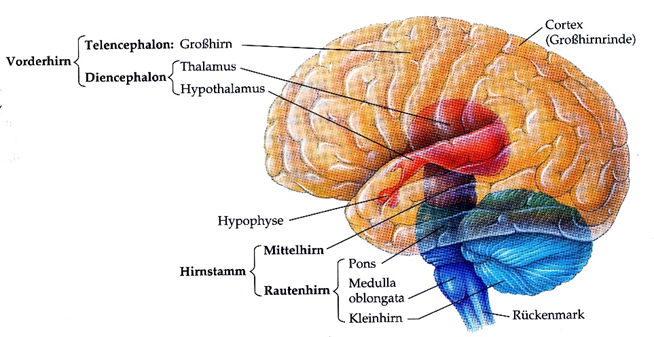
\includegraphics[width=0.8\textwidth]{abbildungen/anatomieNBG.png} % Lädt das Bild, skaliert es auf 80% der Textbreite
%	\caption{ Aufbau des Gehirns \parencite{MarklBild1997a}} % Die Bildunterschrift
%	\label{fig:anaNBG} % Ein Label für Querverweise (z.B. "siehe Abbildung \ref{fig:beispielbild}")
%\end{figure}
%
%Das Kleinhirn liegt hinter bzw.\ unter dem Großhirn. Seine
%Hauptfunktion liegt in der Koordination von Bewegungen. So enthält es
%beispielsweise Informationen zur Stellung der Gelenke oder Länge der
%Muskeln und kann, nach Input des Großhirns über motorische Ausgänge, die
%automatische Koordination von Körperbewegungen und die Balance steuern.
%Durch das Kleinhirn wird also ein fließender und abgestimmter
%Bewegungsablauf ermöglicht, der zum Beispiel bei der
%Auge-Hand-Koordination von Bedeutung
%ist.\footcite[S.~1106]{Markl1997}
%
%Einige Teile des Zwischenhirns und des Großhirns bilden das
%limbische System, das unter anderem den Hippocampus umfasst.
%Der Hippocampus ist eine paarig angelegte Struktur. Er befindet
%sich am Innenrand des Temporallappens und an den Seitenventrikeln. Der
%Hippocampus spielt eine entscheidende Rolle bei der Gedächtnisbildung.
%Insbesondere ist er an der Konsolidierung von Gedächtnisinhalten
%beteiligt, also an der Überführung neuer Informationen aus dem
%Kurzzeitgedächtnis in das Langzeitgedächtnis. Darüber hinaus ist er von
%Bedeutung für das räumliche Gedächtnis sowie für Lernprozesse. Durch
%seine Einbindung in das limbische System ist er ebenfalls an Funktionen
%wie Emotionen und Motivation
%beteiligt.\footcite{Hoegemann2006}
%
%Das periphere Nervensystem bildet den zweiten großen Bestandteil
%des menschlichen Nervensystems. Topografisch gliedert es sich in die
%Hirnnerven und die Spinalnerven. Der Mensch besitzt zwölf
%Hirnnervenpaare, welche direkt aus dem Gehirn austreten und vor allem
%den Kopf- und Halsbereich versorgen, sowie 31 Spinalnervenpaare, die aus
%dem Rückenmark hervorgehen und in den Rumpf, die Extremitäten und die
%inneren Organe führen. Diese peripheren Nerven bestehen jeweils
%aus Bündeln vieler Neuronen. Das periphere Nervensystem setzt sich aus
%zwei funktionellen Untereinheiten zusammen. Die sensorische Untereinheit
%leitet Informationen von Sinneszellen oder inneren Organen zum zentralen
%Nervensystem. Dies findet beispielsweise bei dem Registrieren von Wärme
%oder Kälte statt. Die motorische Untereinheit hingegen überträgt Signale
%aus dem zentralen Nervensystem an die Effektoren, also zu Muskel- oder
%Drüsenzellen. Der motorische Anteil des peripheren Nervensystems kann
%weiter in das somatische und das autonome Nervensystem gegliedert
%werden, wobei das somatische Nervensystem bewusste Bewegungen steuert,
%während das autonome Nervensystem durch das Zusammenwirken von
%Sympathicus und Parasympathicus unwillkürliche Prozesse wie
%beispielsweise den Herzschlag
%reguliert.\footcite[S.~1100--1102]{Markl1997}


\subsection{Signalweiterleitung am Axon und synaptische Signalübertragung}

Um die Rolle bestimmter Proteine für die Signalweiterleitung in einer
Nervenzelle zu verstehen, sollen der Aufbau einer Nervenzelle sowie der
Prozess der Signalweiterleitung genauer betrachtet werden.

Die grundlegende Funktionseinheit des Nervensystems ist die
Nervenzelle, auch Neuron genannt.

\begin{figure}[h] % [h] versucht, das Bild hier zu platzieren (hier), [t] für oben, [b] für unten
	\centering % Zentriert das Bild horizontal
	
\includegraphics[width=0.7\textwidth]{NEU1bild.jpg} % Lädt das Bild, skaliert es auf 80% der Textbreite
	\caption{ Aufbau einer Nervenzelle \parencite{MediKarriere2024}} % Die Bildunterschrift
	\label{fig:NEU1} % Ein Label für Querverweise (z.B. "siehe Abbildung \ref{fig:beispielbild}")
\end{figure}

Ein Neuron besteht aus einem Zellkörper (Soma), welcher das Zellplasma,
den Zellkern sowie weitere typische Zellorganellen enthält. (Zwischen dem Zellinneren und dem äußeren Milieu gibt es unterschiedliche Ionenzusammensetzungen, die zum Teil von der Zelle aktiv aufrecht erhalten werden. (Durch die unterschiedlichen positiven und negativen Ladungen und den chemischen Gradienten entsteht an der Membran ein Potential, das Membranpotential). Das Zellinnere ist dabei im Vergleich zum Zelläußeren negativ geladen, das Zelläußere positiv.) Vom Zellkörper gehen Dendriten, verzweigte Fortsätze des Neurons, aus, die der
Aufnahme eingehender Signale anderer Neuronen dienen. Sie leiten Signale
elektrisch zum Zellkörper weiter. Am Übergang zum Axon, dem Axonhügel,
werden die eingehenden Signale summiert.  Über das Axon werden elektrische Spannungsänderungen bis zu den synaptischen Endigungen weitergeleitet. Dort wird das ankommende elektrische Signal in ein chemisches Signal umgewandelt, indem Neurotransmitter in den synaptischen Spalt ausgeschüttet werden. Auf
diese Weise wird die Information auf eine nachgeschaltete Nerven-,
Muskel- oder Drüsenzelle
übertragen.\footcite[S.~1082--1083]{Markl1997}

Ein Aktionspotential (vgl. Abb \ref{fig:APbild}) ist eine ein bis zwei Millisekunden anhaltende,
markante Änderung des Membranpotentials der
Zellmembran.\footcite{Hircin2007}

Das Membranpotential ist die elektrische Spannung, die zwischen der
Außen- und Innenseite der Zellmembran, aufgrund von
Ladungsunterschieden,
besteht.\footcite{AntwerpesMembranpotential2006}

Alle Zellen bilden ein solches Membranpotential aus, jedoch können
Neuronen ihr Membranpotential aktiv verändern. Man bezeichnet sie daher
auch als erregbare Zellen. Im Ruhezustand weist die Membran der
Nervenzelle ein negatives Ruhepotential auf, das ca.\
$-70$~Millivolt (mV) beträgt. Wird am Axonhügel der Zelle durch das
Summieren der eingehenden Signale ein bestimmter Schwellenwert
überschritten, welcher in der Regel bei $-55$~mV liegt, kommt es zur
Öffnung spannungsgesteuerter Natriumionenkanäle. Der darauffolgende
Einstrom von positiv geladenen Natriumionen in das Zellinnere führt zu
einer Depolarisation, also einer Verschiebung des Membranpotentials in
den positiven Bereich. Diese Depolarisation bewirkt die Öffnung weiterer
Natriumionenkanäle, wodurch das Innere der Zelle rasant positiver wird.
Dieser Vorgang folgt dem Prinzip der positiven Rückkopplung. Während
sich die spannungsgesteuerten Natriumionenkanäle bei einer
Depolarisation sehr schnell öffnen, gibt es eine zeitliche Verzögerung bis zur Öffnung der spannungsgesteuerten Kaliumionenkanäle.
Infolgedessen strömen Kaliumionen aus dem Zellinneren in den
extrazellulären Raum. Da die Natriumionenkanäle bereits wieder
geschlossen sind, führt der Ausstrom der Kaliumionen zur Repolarisation
der Membran. Durch ein verzögertes Schließen der Kaliumionenkanäle strömen eine kurze Zeit nach dem Erreichen eines Membranpotentials von -70 mV weitere Kaliumionen nach außen, was eine Hyperpolarisation bewirkt. (Während der Hyperpolarisation kann die Zelle nicht erregt werden. Diese Zeit nennt man auch Refraktärzeit.) Die Natrium-Kalium-Pumpe stellt anschließend das ursprüngliche,, negative Ruhepotential wieder her.\footcite[S.~1087--1089]{Markl1997}

\begin{figure}[h] % [h] versucht, das Bild hier zu platzieren (hier), [t] für oben, [b] für unten
	\centering % Zentriert das Bild horizontal
	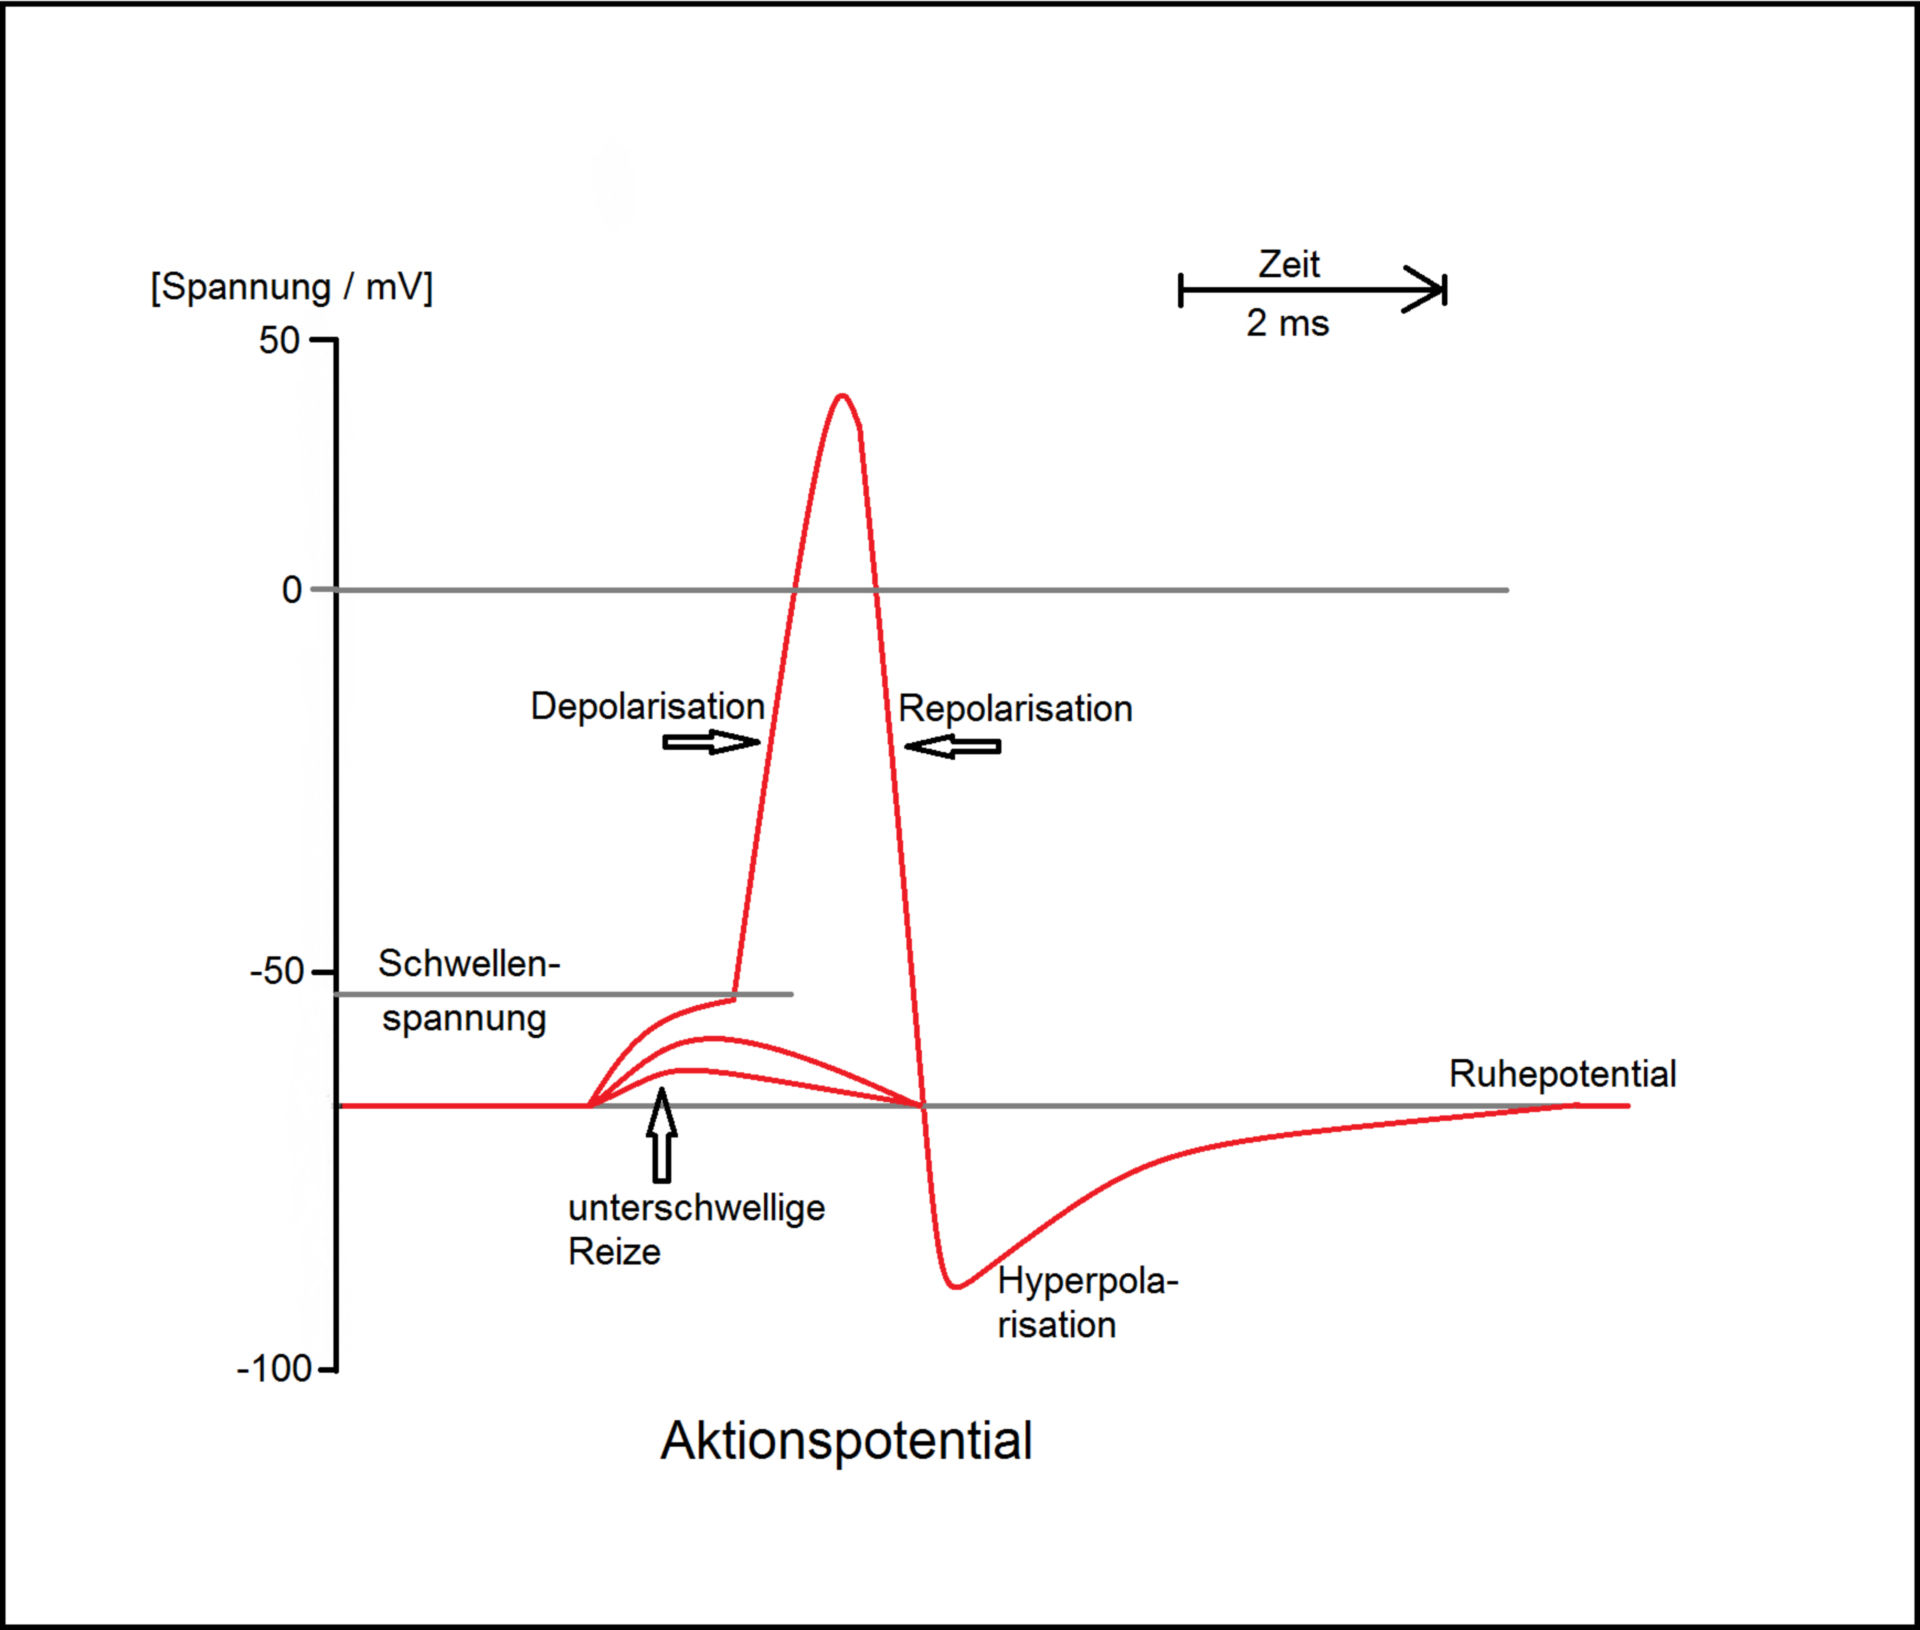
\includegraphics[width=0.8\textwidth]{abbildungen/APbild.jpg} % Lädt das Bild, skaliert es auf 80% der Textbreite
	\caption{UNterschrift nötig \parencite{DocCheckAPBIld}
	} % Die Bildunterschrift
	\label{fig:APbild} % Ein Label für Querverweise (z.B. "siehe Abbildung \ref{fig:beispielbild}")
\end{figure}

Das Aktionspotential breitet sich anschließend entlang des Axons aus.
Das Axon ist häufig von einer Myelinscheide umgeben, die von spezialisierten Gliazellen gebildet wird. Die Myelinscheide dient als elektrische Isolierung und ist in
regelmäßigen Abständen durch Ranvier-Schnürringe unterbrochen
(siehe Abbildung \ref{fig:salaNBG}). Die spannungsgesteuerten Natrium- und
Kaliumionenkanäle sind dabei überwiegend an den Ranvier-Schnürringen
konzentriert. Eine Depolarisation, die durch ein Aktionspotential an
einem Ranvier-Schnürring ausgelöst wurde, breitet sich im Zellplasma
aus und führt auch am nächsten Ranvier-Schnürring zur Öffnung
spannungsgesteuerter Natriumionenkanäle. Dort wird nach dem zuvor
beschriebenen Prinzip erneut ein Aktionspotential ausgelöst. Das Aktionspotential wird also durch die spannungsgesteuerten
Ionenkanäle sequenziell nur an den Ranvier-Schnürringen neu generiert und so entlang des Axons bis zu den
synaptischen Endigungen weitergeleitet, wobei die spannungsgesteuerten
Kaliumionenkanäle für die Repolarisation verantwortlich sind. Dies
bezeichnet man als saltatorische
Erregungsleitung.\footcite[S.~1090--1091]{Markl1997}

% ── Abbildung 3 ausgelassen ──────────────────────────────────
% Abbildung 3: Saltatorische Erregungsweiterleitung
% Quelle: \cite[S.~1091]{Markl1997}
% ─────────────────────────────────────────────────────────────
\begin{figure}[h] % [h] versucht, das Bild hier zu platzieren (hier), [t] für oben, [b] für unten
	\centering % Zentriert das Bild horizontal
	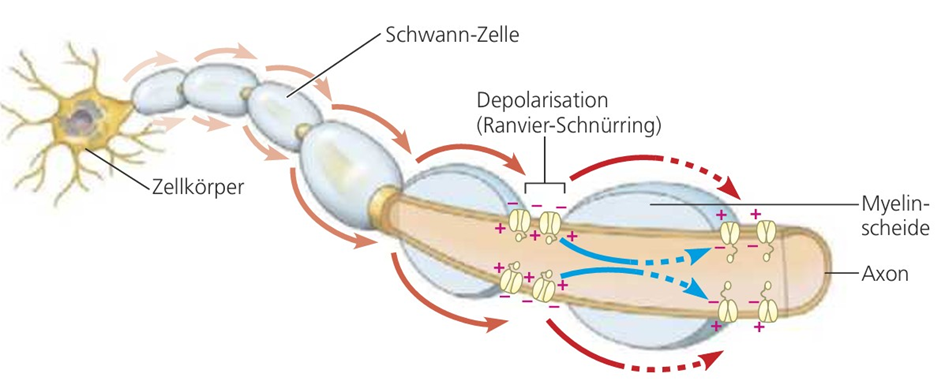
\includegraphics[width=0.8\textwidth]{abbildungen/SaltatorischeNBG.png} % Lädt das Bild, skaliert es auf 80% der Textbreite
	\caption{Saltatorische Erregungsweiterleitung \parencite{MarklBild1997b}
	} % Die Bildunterschrift
	\label{fig:salaNBG} % Ein Label für Querverweise (z.B. "siehe Abbildung \ref{fig:beispielbild}")
\end{figure}


Trifft ein Aktionspotential an der präsynaptischen Endigung ein, kommt
es zur Depolarisation der Membran, was zur Öffnung
spannungsgesteuerter Calciumionenkanäle führt. Der folgende Einstrom von
Calciumionen führt zur Fusion der synaptischen Vesikel mit der Membran
und zur Freisetzung von Neurotransmittern in den synaptischen Spalt. (siehe Abbildung 2.4)
\clearpage

% ── Abbildung 4 ausgelassen ──────────────────────────────────
% Abbildung 4: Aufbau und Funktionsweise einer chemischen Synapse
% Quelle: \cite{DocCheckSynapse2026}
% ─────────────────────────────────────────────────────────────
\begin{figure}[h] % [h] versucht, das Bild hier zu platzieren (hier), [t] für oben, [b] für unten
	\centering % Zentriert das Bild horizontal
	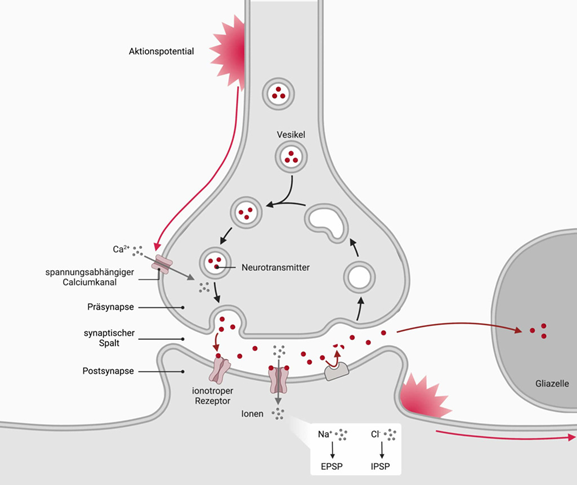
\includegraphics[width=0.7\textwidth]{abbildungen/chemsynapseNBG.png} % Lädt das Bild, skaliert es auf 80% der Textbreite
	\caption{Aufbau und Funktionsweise einer chemischen Synapse \parencite{DocCheckSynapseBild2026}
	} % Die Bildunterschrift
	\label{fig:chemNNBG} % Ein Label für Querverweise (z.B. "siehe Abbildung \ref{fig:beispielbild}")
\end{figure}

Spannungsabhängige Kaliumionenkanäle des Typs Kv1 spielen eine wichtige
Rolle bei der Repolarisation der Membran. Sie begrenzen auch hier die
Dauer des Aktionspotentials und dadurch den Calciumioneneinstrom. So
beeinflussen sie indirekt die Menge an freigesetzten Neurotransmittern.
Je nach Art der freigesetzten Neurotransmitter unterscheidet man
erregende und hemmende Synapsen. Zum Beispiel ist Glutamat ein wichtiger
erregender (exzitatorischer) Transmitter. Für den Transport von Glutamat
in die synaptischen Vesikel ist das Vesikelprotein VGlut1 (Vesikulärer
Glutamat-Transporter~1) verantwortlich. Daher dient VGlut1 als Marker
für exzitatorische Synapsen. Das Protein VGat (Vesikulärer
GABA/Glyzin-Transporter) hingegen transportiert inhibitorische
Neurotransmitter wie Gammaaminobuttersäure (GABA) in die Vesikel und ist
somit ein Marker für hemmende
Synapsen.\footcite[S.~1092]{Markl1997}

% ── Abbildung 6 ausgelassen ──────────────────────────────────
% Abbildung 6: Domänenorganisation von Caspr2
% Quelle: \cite{Canali2018}
% ─────────────────────────────────────────────────────────────
\clearpage